\documentclass[Thesis.tex]{subfiles}
\begin{document}
\chapter{Monte Carlo Methods}
\label{chp:monte-carlo}

\glsreset{pdf}

In \cref{chp:variational-monte-carlo} we found that we needed a way to sample
system configurations $\vX$ from the \gls{pdf} described by the
wave function. We needed this as a means to evaluate integrals. Specifically, we
needed to evaluate the expectation value of the Hamiltonian w.r.t. a given wave
function $\psialpha$:

\begin{align}
    \expval{\hat H} &= \frac{\expval{\hat H}{\psialpha}}{\braket{\psialpha}} = \int\dd{\vX} P_{\psi_{\valpha}} (\vX) E_L(\vX)\label{eq:chp-mc-anon-1}\\
    &\approx \frac{1}{N} \sum_{i = 1}^N E_L(\vX_i)
    \qq{where} \vb X_i\disteq P_{\psi_{\valpha}}.
\end{align}
where $N$ is set sufficiently large to satisfy the required accuracy. Due to
the central nature of this method, we will start by a proper presentation of
this \gls{mc} technique as it is used here, followed the details of how to
obtain the samples we need.

\section{Monte Carlo Integration}

\acrfull{mci} is a general technique for numeric evaluation of
any arbitrary integral. In general it concerns evaluating any multidimensional
definite integral, written as:

\begin{align}
    I = \idotsint_\sigma\dd{\vx} f(\vx),
\end{align}
for some integrand $f(\vx)$ and where $\sigma$ denotes a subset of $\mathbb{R}^m$ with a $m$-dimensional volume given by:
\begin{align}
    V = \idotsint_\sigma\dd{\vx}
\end{align}
In its simplest form, \gls{mci} works by sampling $N$ \emph{uniformly} distributed points
$\vx_1,\dots,\vx_N$ from $\sigma$, and uses a Riemann sum formulation of the
integral $I$:\footnote{Notice that $\vx_i$ now denotes one random sample, and
  has nothing to do with the $i$'th particle. For the time being we don't talk
  about particles, and the subscripts indicate different samples.}
\begin{align}
  \label{eq:mci-def}
    I = \lim_{N\to\infty} M_N \defeq \lim_{N\to\infty}\sum_{i=1}^N f(\vx_i) \frac{V}{N} = V\expval{f(\vx)}_\sigma,
\end{align}
where $\expval{\cdot}_\sigma$ denotes the expectation value over all points in
$\sigma$ when all points are equally likely. The estimate becomes increasingly
accurate for increasing $N$, and is exact in the limit where $N\to\infty$.

\subsection{Estimating the Error}

For any finite $N$ the result of using \gls{mci} will not be exact. Because of
this, it is immensely useful to be able to assign a statistical certainty to the
result. For instance, say we estimate the ground state energy of a system using
two different wave functions. We perform the integrals and get (to the first
five digits) $\expval{H}_A = \SI{1.0315}{eV}$ and $\expval{H}_B =
\SI{1.0943}{eV}$. Recalling that the lowest energy is the most physically
accurate, can we say that $A$ is better than $B$? No, because we lack
information on the precision of the integrals. Assume that in reality, the
numbers were $\expval{H}_A=\SI{1.03(8)}{eV}$ and
$\expval{H}_B=\SI{1.09(8)}{eV}$, where the numbers in parenthesis indicate the
uncertainty in the last digit. Now we know that the two numbers are not
different in a statistically significant way, and any difference could be
entirely random. We would need to use more sample points to lower the
uncertainty to be able to say anything more about them.\\

We obtain a statistical estimate of the error we make in approximating the
integral by considering the variability of the individual terms of
\cref{eq:mci-def}. Let's start by estimating the variance of the integrand:
\begin{align}
    \Var[f(\vx)] \defeq \sigma^2_N = \frac{1}{N-1} \sum_{i=1}^N\qty(f(\vx_i) - \frac{1}{N}\sum_{j=1}^N f(\vx_j))^2.
\end{align}
It then follows, by the properties of variance,
\begin{align}
  \label{eq:mci-annon-2}
    \Var[M_N] = \Var\qty[ \frac{V}{N} \sum_{i=1}^Nf(\vx_i)] = \frac{V^2}{N^2}\sum_{i=1}^N\Var[f(\vx_i)] = \frac{V^2\sigma^2_N}{N}
\end{align}
\begin{align}
  \label{eq:mci-sem-def}
    \implies \Std[M_N] = \sqrt{\Var[M_N]} = \frac{V\sigma_N}{\sqrt N}.
\end{align}
\Cref{eq:mci-sem-def} is the standard deviation of the sample mean, otherwise
known as the \gls{sem}. It is common use the \gls{sem} as the estimate of uncertainty on
expectation values. Another common choice is to give confidence intervals
based on the \gls{sem}. Assuming the variance is normally
distributed,\footnote{Which for our wave functions is often times at least
  approximately true.} we can say with e.g.\ $\SI{95}{\percent}$ certainty that
the true expectation value, I, is in the interval

\begin{align}
  \qty[CI_{-}^{95}, CI_{+}^{95}] \defeq \qty[M_N - 1.96\Std[M_N], M_N + 1.96\Std[M_N]].
\end{align}

\Cref{eq:mci-sem-def} tells us that the expected statistical error we make when using \gls{mci} goes
like $\mathcal{O}(1 / \sqrt N)$, and depends linearly on the size of the volume
and standard deviation of the integrand itself. This illustrates both the
advantage, and disadvantage of \gls{mci} compared to other,
deterministic integration methods. Its advantage is its simple dependency on the
volume, and its independence from the particular number of dimensions in the
integral. Other methods tend to depend exponentially on the dimensionality, and
as such \gls{mci} is often the best choice for multidimensional integrals. Its
disadvantage is the relatively slow convergence rate, which is asymptotically
much worse than other approaches~\cite{Numerical-Recipes-Press-et-al}.

\subsubsection{Correction for Autocorrelation}

Actually, \cref{eq:mci-annon-2} includes a mistake. We applied a property of
variance on a sum of random variables. The equation is correct if and
only if the samples $\vx_i$ are perfectly independent. Unfortunately for us,
the samples will not always be so, depending on the algorithm used to generate
them. We can sample independently from a uniform distribution and some other
notable distributions (\cref{sec:sampling-arb-prob-dist-funcs}), but not in
general. This will be especially true for the algorithms we use to sample from
arbitrary wave functions (\cref{sec:metro-hastings-alg}).

The version of \cref{eq:mci-annon-2} that is true in general accounts for
autocorrelated samples:\footnote{Covariance is a measure of the joint
  variability between two random variables. Autocorrelation is used to refer to
  the covariance between a random variable and itself at pairs of time points.}


\begin{align}
  \label{eq:mci-annon-3}
    \Var[M_N] = \Var\qty[ \frac{V}{N} \sum_{i=1}^Nf(\vx_i)] = \frac{V^2}{N^2}\sum_{i=1}^N\sum_{j=1}^N\Cov[f(\vx_i), f(\vx_j)].
\end{align}
This is always greater than or equal to \cref{eq:mci-annon-2}, and equal only if
the off-diagonal covariance terms (where $i\neq j$) are all zero. Not accounting
for the autocorrelation in the samples will therefore lead us to underestimate
the error, which is arguably much worse than the opposite.

There is, unfortunately a heavy cost to computing the full covariance.
Typically, to keep the expectation values accurate, we will use very large
values for $N$, often on the order of tens or hundreds of millions. The double loop in
\cref{eq:mci-annon-3} will then quickly become unfeasible to compute, with
trillions or quadrillions of iterations. In practice we need to estimate it.
Yes, we are going to estimate the estimate of the error we make in an estimate.

The strategy we shall use for all later error analysis is called \emph{blocking},
and specifically we use an automated form presented in an article by
\textcite{Jonsson-2018}. Say we have a sequence of sample values $f(x_i)$:

\begin{align}
  D_0 = \mqty[f(x_1) & f(x_2) & \dots & f(x_N)],
\end{align}
and let's assume that there is some non-zero autocovariance between samples that are
sufficiently close in the sequence. The idea of blocking is to group
\say{blocks} of samples together, replacing them by their mean value. For
instance, after one blocking transformation of the above sequence we get:

\begin{align}
  D_1 = \mqty[\qty(\frac{f(x_1) + f(x_2)}{2}) & \qty(\frac{f(x_3) + f(x_4)}{2}) & \dots & \qty(\frac{f(x_{n-1}) + f(x_n)}{2})].
\end{align}
If $N = 2^d$ with $d > 1$ we can repeat the process to obtain $d$ different
sequences $D_i$. These transformations conserve the value of \cref{eq:mci-annon-3}
while decreasing the covariance between samples~\cite{Jonsson-2018}. That implies that measuring
the variance with \cref{eq:mci-annon-2} on each $D_i$ will yield greater and
greater errors, until there is no more covariance and the error estimate
converges.

\Cref{fig:blocking-example-diagram} shows this process in practice. The example
data is $2^{27}$ samples of the mean radial displacement of a single
one-dimensional particle placed in a harmonic oscillator. Due to how the data is
generated, we expect there to be a significant portion of autocorrelation
present. The figure shows the standard error from \cref{eq:mci-annon-2},
calculated on the data sets obtained by performing repeated blocking
transformations. We can see it rises steadily during the first $6$-$7$
transformations, after which the block sizes are big
enough to remove all the covariance and the estimate converges. As
the data set becomes too small the results start to become unpredictable. The
optimal estimate is indicated by the red circle, as determined by the automated
procedure developed by \textcite{Jonsson-2018}. In this particular case this occurred after
$\num{12}$ blocking transformations.

If not explicitly stated otherwise, all error estimates in this thesis will
include this correction.


\begin{figure}[h]
  \centering
  \resizebox{0.7\linewidth}{!}{%
    % This file was created by matplotlib2tikz v0.7.4.
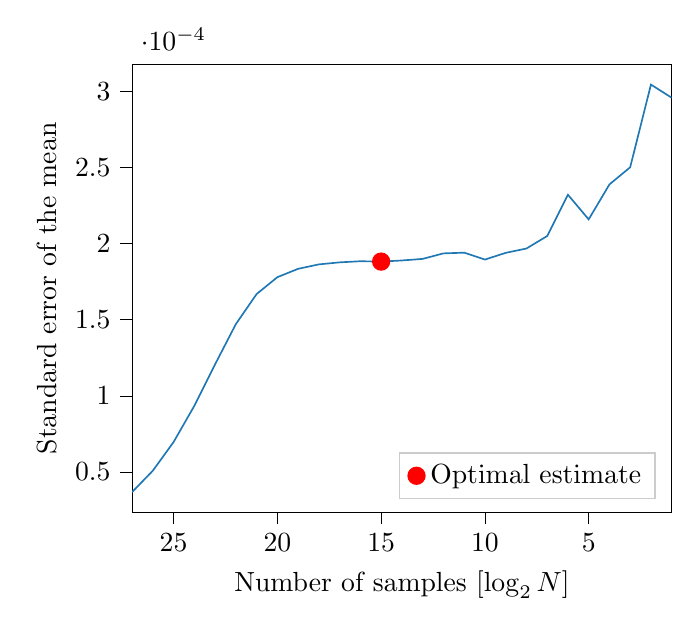
\begin{tikzpicture}

\definecolor{color0}{rgb}{0.12156862745098,0.466666666666667,0.705882352941177}

\begin{axis}[
legend cell align={left},
legend style={at={(0.97,0.03)}, anchor=south east, draw=white!80.0!black},
tick align=outside,
tick pos=left,
x grid style={white!69.01960784313725!black},
xlabel={Number of samples [\(\displaystyle \log_2 N\)]},
xmin=1, xmax=27,
x dir=reverse,
xtick style={color=black},
y grid style={white!69.01960784313725!black},
ylabel={Standard error of the mean},
ymin=2.34108439617707e-05, ymax=0.000317790214944944,
ytick style={color=black}
]
\addplot [semithick, color0, forget plot]
table {%
27 3.67917244610058e-05
26 5.08561376062952e-05
25 6.96692672721627e-05
24 9.34552651332882e-05
23 0.000120713739651834
22 0.000147100021974398
21 0.000166850831566622
20 0.000177932968353421
19 0.000183425162994512
18 0.000186334983085339
17 0.000187672447620898
16 0.000188413104177414
15 0.000188165276488921
14 0.000188912298901297
13 0.000189945032792876
12 0.000193566076049745
11 0.000194033153176985
10 0.000189501762734578
9 0.000193910232467662
8 0.000196755580260382
7 0.000204949815919038
6 0.000232063166781732
5 0.000215889931697987
4 0.000238840926305042
3 0.000250129403607225
2 0.000304409334445708
1 0.000295753527333449
};
\addplot [semithick, red, mark=*, mark size=3, mark options={solid}, only marks]
table {%
15 0.000188168147728901
};
\addlegendentry{Optimal estimate}
\end{axis}

\end{tikzpicture}
  }
  \caption[Standard error as a function of blocking transformations]{The estimated standard error of a random process excibiting symptoms
    of autocorrelation, shown as a function of the effective size of the data set as
    blocking transformations are applied. As the block sizes increase the
    covariance goes away, while the variance increases. After convergence, the
    optimal estimate is illustrated by the red dot, as determined by an automated blocking
    procedure~\cite{Jonsson-2018}.\citesource{writing/scripts/blocking-example-diagram.py}}
  \label{fig:blocking-example-diagram}
\end{figure}



\subsection{Importance Sampling}

In some suitable cases we can improve quite dramatically on the simple,
straightforward integration approach given in \cref{eq:mci-def} with a technique
known as \gls{is}. To illustrate this, say we
would like to evaluate the following integral:

\begin{align}
    \label{eq:mci-importance-example-func}
    I = \intfy\dd{x}f(x)=\intfy\dd{x} \frac{\exp{-\flatfrac{x^2}{2} }}{\sqrt{2\pi \qty(1 +x^2)}}  = \num{0.78964}.
\end{align}

\begin{figure}
    \centering
    \resizebox{0.7\linewidth}{!}{%
    \begin{tikzpicture}
        \begin{axis}[every axis plot post/.append style={
                mark=none,domain=-5:5,samples=50,smooth}, % All plots: from -2:2, 50 samples, smooth, no marks
            axis x line=bottom, % no box around the plot, only x and y axis
            axis y line=left,
            enlargelimits=upper] % extend the axes a bit to the right and top
            \addplot[semithick, color0] {1/(sqrt(2*pi))*exp(-(x^2)/2)*(1+x^2)^(-0.5)};
            \addplot[semithick, color1] {1/(sqrt(2*pi))*exp(-(x^2)/2)};
            \addlegendentry{$f(x)$}
            \addlegendentry{$\mathcal{N}(0, 1)$}
        \end{axis}
    \end{tikzpicture}
    }
    \caption[Illustration of example probability distributions]{\label{fig:mci-importance-example-func-plot}Plot of the function in
      \cref{eq:mci-importance-example-func}, enveloped by a standard normal distribution.\citesource{writing/MonteCarlo.tex}}
\end{figure}
\noindent The integrand is plotted in \cref{fig:mci-importance-example-func-plot}, and
the observant reader might recognise this as the product of a normal
distribution and a Student-t distribution. The correct value for the integral
is also given, so we have a reference for the results.

For comparison, let's start with the straightforward approach from before.
Because the integral goes to infinity the "volume" $V$ would not be well
defined, and we are forced to truncate the region manually. From looking at the
graph in \cref{fig:mci-importance-example-func-plot} we may say that $x\in
[-5, 5]$ should account for the vast majority of the total integral. That means
we use the following estimate:

\begin{align}
    \label{eq:chp-mc-anon-2}
    I\approx \frac{10}{N}\sum_{i=1}^Nf(x_i)\qq{where} x_i\disteq\text{Uniform}(-5, 5).
\end{align}

\noindent The main issue with this approach is that 1) we need to truncate the integral
manually and 2) no matter where we place the box boundaries we will tend to
sample a lot of $x_i$'s in areas where $f$ gives very small contributions to
the integral. Ideally we would like our sample points to be distributed as
closely as possible to $f$, in order to capture as much information as we can.
This is the idea of \gls{is}. Instead of using the uniform
distribution for sampling, we use some probability distribution which more
closely resembles the integrand, call it $g(x)$. Formally we then restate the integral as follows:

\begin{align}
    I = \intfy\dd{x}f(x) = \intfy\dd{x} \frac{f(x)}{g(x)} g(x).
\end{align}
This can be interpreted as the expectation of $z(x)=\flatfrac{f(x)}{g(x)}$ for $x$'s drawn from $g$, and so the corresponding estimation is then:

\begin{align}
    I \approx \frac{1}{N} \sum_{i=1}^N \frac{f(x_i)}{g(x_i)} \qq{where} x_i\disteq g.
\end{align}
Setting $g = \text{Uniform}(-5, 5)$ recovers \cref{eq:chp-mc-anon-2}, so this is
simply the natural generalization of the standard approach for an arbitrary
\gls{pdf}.


Going back to the example, we should now choose a distribution function that
closely resembles the integrand, while still being simple to sample from. In
this (contrived) example, a natural choice is to use the standard normal
distribution, $g = \mathcal{N}(0, 1)$. In
\cref{fig:mci-importance-example-func-plot} we can see how $g(x)$ is
enclosing $f(x)$ much more tightly than any rectangular box might hope to.

\begin{figure}
   \centering
    \resizebox{0.7\linewidth}{!}{%
        % This file was created by matplotlib2tikz v0.7.4.
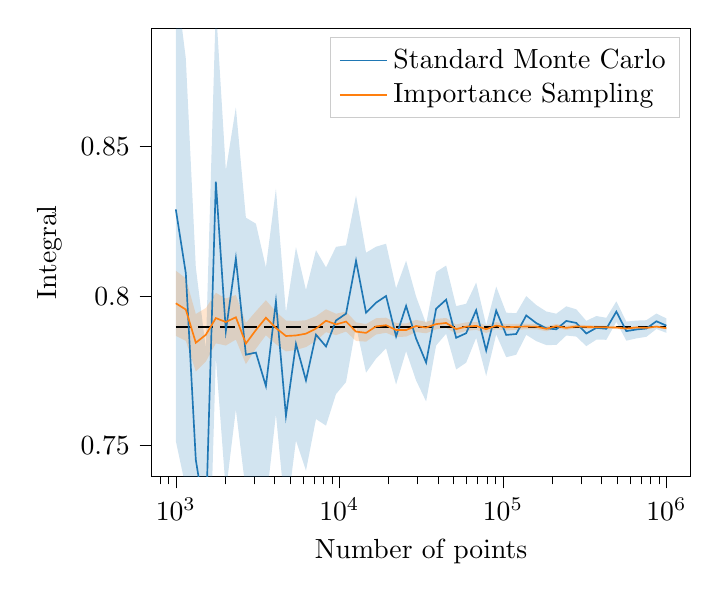
\begin{tikzpicture}

\definecolor{color0}{rgb}{0.12156862745098,0.466666666666667,0.705882352941177}
\definecolor{color1}{rgb}{1,0.498039215686275,0.0549019607843137}

\begin{axis}[
legend cell align={left},
legend style={draw=white!80.0!black},
log basis x={10},
tick align=outside,
tick pos=left,
x grid style={white!69.01960784313725!black},
xlabel={Number of points},
xmin=707.945784384138, xmax=1412537.54462276,
xmode=log,
xtick style={color=black},
y grid style={white!69.01960784313725!black},
ylabel={Integral},
ymin=0.73964, ymax=0.88964,
ytick style={color=black}
]
\path [fill=color0, fill opacity=0.2]
(axis cs:1000,0.906505519198725)
--(axis cs:1000,0.751532172525837)
--(axis cs:1151,0.735831543753176)
--(axis cs:1325,0.680849621063098)
--(axis cs:1526,0.66635670415917)
--(axis cs:1757,0.779382816946574)
--(axis cs:2023,0.734566699673617)
--(axis cs:2329,0.762035463989511)
--(axis cs:2682,0.734565832804202)
--(axis cs:3088,0.73798169568494)
--(axis cs:3556,0.730217784390541)
--(axis cs:4094,0.760469759098198)
--(axis cs:4714,0.725360612203807)
--(axis cs:5428,0.751700043683699)
--(axis cs:6250,0.741602925670416)
--(axis cs:7196,0.758867234301727)
--(axis cs:8286,0.756687693428198)
--(axis cs:9540,0.767228880540759)
--(axis cs:10985,0.771229626136113)
--(axis cs:12648,0.790012094541718)
--(axis cs:14563,0.774391523089762)
--(axis cs:16768,0.77909942060995)
--(axis cs:19306,0.782536739216005)
--(axis cs:22229,0.770428521449884)
--(axis cs:25595,0.781574784789273)
--(axis cs:29470,0.771759717058446)
--(axis cs:33932,0.764776709236966)
--(axis cs:39069,0.783487769922224)
--(axis cs:44984,0.787414355694207)
--(axis cs:51794,0.775475553467901)
--(axis cs:59636,0.777740489465899)
--(axis cs:68664,0.786049955378521)
--(axis cs:79060,0.773275873950683)
--(axis cs:91029,0.787160195206047)
--(axis cs:104811,0.779567528991012)
--(axis cs:120679,0.780390365577674)
--(axis cs:138949,0.787053593717609)
--(axis cs:159985,0.784957670264303)
--(axis cs:184206,0.783635621994808)
--(axis cs:212095,0.783663303380307)
--(axis cs:244205,0.786824569813399)
--(axis cs:281176,0.786472339541122)
--(axis cs:323745,0.783270774763061)
--(axis cs:372759,0.785431295025521)
--(axis cs:429193,0.785403139227959)
--(axis cs:494171,0.79137576492629)
--(axis cs:568986,0.785095481165753)
--(axis cs:655128,0.785862960669846)
--(axis cs:754312,0.786388810526214)
--(axis cs:868511,0.789001256366245)
--(axis cs:1000000,0.78771906388357)
--(axis cs:1000000,0.792542831612807)
--(axis cs:1000000,0.792542831612807)
--(axis cs:868511,0.794181220859291)
--(axis cs:754312,0.791942882951014)
--(axis cs:655128,0.791820110680025)
--(axis cs:568986,0.791487504496917)
--(axis cs:494171,0.798260611327551)
--(axis cs:429193,0.792759708194515)
--(axis cs:372759,0.793337949884088)
--(axis cs:323745,0.791729598374579)
--(axis cs:281176,0.795583619643708)
--(axis cs:244205,0.796589010550667)
--(axis cs:212095,0.79412837031455)
--(axis cs:184206,0.794870279758202)
--(axis cs:159985,0.79701634187077)
--(axis cs:138949,0.800016332107068)
--(axis cs:120679,0.794272570875621)
--(axis cs:104811,0.794468511086953)
--(axis cs:91029,0.803200188932203)
--(axis cs:79060,0.790355947691124)
--(axis cs:68664,0.804549926843196)
--(axis cs:59636,0.797454867544406)
--(axis cs:51794,0.796653185040259)
--(axis cs:44984,0.810244363594127)
--(axis cs:39069,0.808073653372737)
--(axis cs:33932,0.790777573023198)
--(axis cs:29470,0.799841366593076)
--(axis cs:25595,0.811867722605131)
--(axis cs:22229,0.802618543013231)
--(axis cs:19306,0.817530506209257)
--(axis cs:16768,0.816541914366059)
--(axis cs:14563,0.814542168015885)
--(axis cs:12648,0.833651170719542)
--(axis cs:10985,0.817018107595682)
--(axis cs:9540,0.816494291003619)
--(axis cs:8286,0.809610747560487)
--(axis cs:7196,0.815367040536989)
--(axis cs:6250,0.802025469808376)
--(axis cs:5428,0.816380403842103)
--(axis cs:4714,0.79455756611557)
--(axis cs:4094,0.83595037286634)
--(axis cs:3556,0.809617017360876)
--(axis cs:3088,0.824249680097279)
--(axis cs:2682,0.826250438806259)
--(axis cs:2329,0.863177790933464)
--(axis cs:2023,0.842110084892558)
--(axis cs:1757,0.897157433940518)
--(axis cs:1526,0.782467186210373)
--(axis cs:1325,0.809627874200951)
--(axis cs:1151,0.879506727836154)
--(axis cs:1000,0.906505519198725)
--cycle;

\path [fill=color1, fill opacity=0.2]
(axis cs:1000,0.808499519570512)
--(axis cs:1000,0.786713211329766)
--(axis cs:1151,0.785042642420524)
--(axis cs:1325,0.774788109289872)
--(axis cs:1526,0.778119575109797)
--(axis cs:1757,0.784198893001299)
--(axis cs:2023,0.783474555689343)
--(axis cs:2329,0.785454412684189)
--(axis cs:2682,0.777230046137711)
--(axis cs:3088,0.782391418189927)
--(axis cs:3556,0.786909552632689)
--(axis cs:4094,0.783902603834432)
--(axis cs:4714,0.781495885789912)
--(axis cs:5428,0.781995739197111)
--(axis cs:6250,0.782947354122917)
--(axis cs:7196,0.785013543050367)
--(axis cs:8286,0.787948023436544)
--(axis cs:9540,0.786939718155325)
--(axis cs:10985,0.78813969801641)
--(axis cs:12648,0.785009178650894)
--(axis cs:14563,0.784773520932163)
--(axis cs:16768,0.787148101226365)
--(axis cs:19306,0.787741557498044)
--(axis cs:22229,0.786316999755659)
--(axis cs:25595,0.786450329615228)
--(axis cs:29470,0.787955851294709)
--(axis cs:33932,0.78757265986175)
--(axis cs:39069,0.788869680545658)
--(axis cs:44984,0.78938055958093)
--(axis cs:51794,0.787415451512896)
--(axis cs:59636,0.788357903529426)
--(axis cs:68664,0.788705910542103)
--(axis cs:79060,0.787681126030283)
--(axis cs:91029,0.78898051397606)
--(axis cs:104811,0.788492546402297)
--(axis cs:120679,0.788732894196601)
--(axis cs:138949,0.788892819560814)
--(axis cs:159985,0.788902704579644)
--(axis cs:184206,0.788249963966235)
--(axis cs:212095,0.789177671294473)
--(axis cs:244205,0.788671473735971)
--(axis cs:281176,0.789205696562338)
--(axis cs:323745,0.789094062911801)
--(axis cs:372759,0.789032879202963)
--(axis cs:429193,0.789047047758369)
--(axis cs:494171,0.789002100901894)
--(axis cs:568986,0.788704796739401)
--(axis cs:655128,0.789067389752803)
--(axis cs:754312,0.788974080074391)
--(axis cs:868511,0.78943145779477)
--(axis cs:1000000,0.788914352720739)
--(axis cs:1000000,0.789617741825269)
--(axis cs:1000000,0.789617741825269)
--(axis cs:868511,0.790185812364)
--(axis cs:754312,0.789784265247556)
--(axis cs:655128,0.789935551227239)
--(axis cs:568986,0.789637087545991)
--(axis cs:494171,0.790002016054565)
--(axis cs:429193,0.790120519045172)
--(axis cs:372759,0.790181903582851)
--(axis cs:323745,0.790329990198755)
--(axis cs:281176,0.790532034926843)
--(axis cs:244205,0.790094903469465)
--(axis cs:212095,0.790704776107281)
--(axis cs:184206,0.789891414252003)
--(axis cs:159985,0.790658336939786)
--(axis cs:138949,0.790774959557188)
--(axis cs:120679,0.790755694443077)
--(axis cs:104811,0.790661819627759)
--(axis cs:91029,0.791309731968405)
--(axis cs:79060,0.790182700029323)
--(axis cs:68664,0.791381769122267)
--(axis cs:59636,0.791238449252401)
--(axis cs:51794,0.790511201000009)
--(axis cs:44984,0.792681004890301)
--(axis cs:39069,0.792413735793226)
--(axis cs:33932,0.791381426805788)
--(axis cs:29470,0.79204983187053)
--(axis cs:25595,0.790859203245189)
--(axis cs:22229,0.79101619799564)
--(axis cs:19306,0.792788925820531)
--(axis cs:16768,0.792596552778913)
--(axis cs:14563,0.790644584700561)
--(axis cs:12648,0.791243995361164)
--(axis cs:10985,0.794832730416374)
--(axis cs:9540,0.794115920221445)
--(axis cs:8286,0.795606481910413)
--(axis cs:7196,0.793283271523529)
--(axis cs:6250,0.791946308583509)
--(axis cs:5428,0.79169137563027)
--(axis cs:4714,0.791830711268204)
--(axis cs:4094,0.794798753178707)
--(axis cs:3556,0.798644174762259)
--(axis cs:3088,0.794920715642714)
--(axis cs:2682,0.791056764105328)
--(axis cs:2329,0.800402702389645)
--(axis cs:2023,0.799215779199193)
--(axis cs:1757,0.801113437531119)
--(axis cs:1526,0.796022529704722)
--(axis cs:1325,0.794032465873107)
--(axis cs:1151,0.805985030304646)
--(axis cs:1000,0.808499519570512)
--cycle;

\path [draw=black, semithick, dash pattern=on 5.550000000000001pt off 2.4000000000000004pt]
(axis cs:1000,0.78964)
--(axis cs:1000000,0.78964);

\addplot [semithick, color0]
table {%
1000 0.829018845862281
1151 0.807669135794665
1325 0.745238747632025
1526 0.724411945184771
1757 0.838270125443546
2023 0.788338392283088
2329 0.812606627461488
2682 0.78040813580523
3088 0.781115687891109
3556 0.769917400875709
4094 0.798210065982269
4714 0.759959089159688
5428 0.784040223762901
6250 0.771814197739396
7196 0.787117137419358
8286 0.783149220494342
9540 0.791861585772189
10985 0.794123866865898
12648 0.81183163263063
14563 0.794466845552823
16768 0.797820667488005
19306 0.800033622712631
22229 0.786523532231558
25595 0.796721253697202
29470 0.785800541825761
33932 0.777777141130082
39069 0.795780711647481
44984 0.798829359644167
51794 0.78606436925408
59636 0.787597678505153
68664 0.795299941110859
79060 0.781815910820903
91029 0.795180192069125
104811 0.787018020038983
120679 0.787331468226647
138949 0.793534962912339
159985 0.790987006067536
184206 0.789252950876505
212095 0.788895836847429
244205 0.791706790182033
281176 0.791027979592415
323745 0.78750018656882
372759 0.789384622454805
429193 0.789081423711237
494171 0.794818188126921
568986 0.788291492831335
655128 0.788841535674935
754312 0.789165846738614
868511 0.791591238612768
1000000 0.790130947748189
};
\addlegendentry{Standard Monte Carlo}
\addplot [semithick, color1]
table {%
1000 0.797606365450139
1151 0.795513836362585
1325 0.784410287581489
1526 0.787071052407259
1757 0.792656165266209
2023 0.791345167444268
2329 0.792928557536917
2682 0.784143405121519
3088 0.788656066916321
3556 0.792776863697474
4094 0.78935067850657
4714 0.786663298529058
5428 0.78684355741369
6250 0.787446831353213
7196 0.789148407286948
8286 0.791777252673478
9540 0.790527819188385
10985 0.791486214216392
12648 0.788126587006029
14563 0.787709052816362
16768 0.789872327002639
19306 0.790265241659288
22229 0.788666598875649
25595 0.788654766430209
29470 0.790002841582619
33932 0.789477043333769
39069 0.790641708169442
44984 0.791030782235616
51794 0.788963326256453
59636 0.789798176390914
68664 0.790043839832185
79060 0.788931913029803
91029 0.790145122972232
104811 0.789577183015028
120679 0.789744294319839
138949 0.789833889559001
159985 0.789780520759715
184206 0.789070689109119
212095 0.789941223700877
244205 0.789383188602718
281176 0.789868865744591
323745 0.789712026555278
372759 0.789607391392907
429193 0.789583783401771
494171 0.78950205847823
568986 0.789170942142696
655128 0.789501470490021
754312 0.789379172660974
868511 0.789808635079385
1000000 0.789266047273004
};
\addlegendentry{Importance Sampling}
\end{axis}

\end{tikzpicture}
    }
    \caption[Convergence of Monte Carlo Integration]{\label{fig:mci-importance-example-func-convergence}Convergence of
    the integral in \cref{eq:mci-importance-example-func}, using regular
    \gls{mci} and \gls{is} with $g = \mathcal{N}(0,
    1)$. The points indicate the approximated value of the integral for each
    particular experiment, and the shaded areas indicate the corresponding
    $\SI{95}{\percent}$ confidence intervals for the expected value. We see the
    latter displaying both greater accuracy and tighter confidence intervals.
    \citesource{writing/scripts/monte_carlo_int_example.py}
    }
\end{figure}

\Cref{fig:mci-importance-example-func-convergence} shows the convergence of
the \gls{mc} approximations towards the correct value for an increasing
number of sampled points. The drawn line is the mean value at each run, while
the shaded areas show the corresponding $\SI{95}{\percent}$ confidence
intervals. Because of the more suited sampling distribution, we obtain results
which are more accurate, and perhaps most importantly, tighter confidence
bounds. In general, using better sampling distributions will tend to give us
lower variance results.

\section{Sampling from Arbitrary Probability Density Functions}
\label{sec:sampling-arb-prob-dist-funcs}

So far we have taken for granted the ability to sample numbers from various
\glspl{pdf}. We dedicate this section to discuss sampling from the bottom up,
culminating in a detailed presentation of the most central algorithm in this
thesis, the Metropolis-Hastings algorithm.

\subsection{The Uniform Distribution}

The basic building block upon which we shall build all other random sampling
techniques is the ability to sample random numbers from the uniform
distribution, $\text{Uniform}(a, b)$. This is the simplest distribution
possible, where all numbers in the range $[a, b]$ have the same probability
density. The definition of its \gls{pdf} is simply:

\begin{align}\label{eq:uniform-pdf-definition}
    p_U\qty(x\;\middle|\; a, b) \defeq  \begin{cases}
        \frac{1}{b - a} &\qfor x\in [a, b]\\
        0&\qotherwise
    \end{cases}.
\end{align}
Most commonly we operate only with the \emph{standard uniform distribution}, $\text{Uniform}(0, 1)$. Any other range can be simply related via the trivially verifiable identity
\begin{align}
    p_U\qty(x\;\middle|\; a,b) = p_U\qty( \frac{x-a}{b-a} \;\middle|\; 0, 1).
\end{align}

But how exactly do we obtain random realizations from this \gls{pdf}? First we need
to depart from the typical notion of randomness, and realize that we are unable to
write an algorithm which produces a truly random result. While we could in
principle rely on nature to provide sources of complete, true randomness (such as
the exact behavior of a quantum mechanical observable), this is impractical
when we need fast, on-demand samples. Instead we settle for
\emph{pseudo-random} samples. A pseudo-random sequence $x_1, x_2,\dots x_n$
implies that one cannot\footnote{In any practical way, barring exhaustive trial
and error of every conceivable underlying algorithm.} predict $x_{n+1}$ without
insight into how the sequence is generated. In other words, the (ideal)
pseudo-random sequence is indistinguishable from a truly random sequence for
anyone observing the numbers $x_i$ alone.

There are a multitude of algorithms that can generate a sequence of
pseudo-random \emph{integers}, all with varying properties.\footnote{Such properties
could include range of possible numbers, period, level of bias and how
cryptographically secure they are.} The simplest family of
such algorithms is a \gls{lcg}~\cite{Knuth-1997-ACP-270146}. It defines a
pseudo-random sequence by the simple recurrence relation
\begin{align}
    \label{eq:linear-congruential-generator-relation}
    x_{n+1} = (ax_n + c)\mod m,
\end{align}
where $a, c$ and $m$ are constants which determine the behaviour of the
algorithm, and $x_0$ needs to be specified manually. For instance,
\textcite{Numerical-Recipes-Press-et-al} use $a = 1664525$, $c=1013904223$ and
$m=2^{32}$.

This produces uniformly distributed integers in the range $[0, m)$. Numbers
from the standard uniform distribution can then simply be obtained by dividing
the integers by $m$. The complete algorithm is shown in \cref{alg:uniform-LCG-sampling}.

\begin{algorithm}[h]
    \caption{Sampling from $\text{Uniform}(l, u)$}
    \label{alg:uniform-LCG-sampling}
    \begin{algorithmic}[1]
        \Require $a, c, m$ and $x_0$
        \Function{unif}{lower bound $l$, upper bound $u$}
            \State $x\gets x_0$
            \Repeat
                \State $x\gets (ax + c)\mod m$
                \State \Yield $(\flatfrac{x}{m}) \times (u - l) + l$
            \Until{done}
        \EndFunction
    \end{algorithmic}
\end{algorithm}

\subsection{Inverse Transform Sampling}

Armed with uniformly distributed random numbers, we now turn towards generating
numbers from other \glspl{pdf}. Let $U\disteq\text{Uniform}(0,1)$ be a uniformly
distributed stochastic variable, and let $X$ be a stochastic variable
associated with a \gls{pdf}, $p$, and a corresponding \gls{cdf}, $F$, i.e.

\begin{align}
    F(x) = \text{Pr}\qty(X\leq x) = \int_{-\infty}^x \dd{t}p(t).
\end{align}
We would like to define a transformation $T:[0, 1]\mapsto\mathbb{R}$ that can map from uniform numbers to numbers that follow the given \gls{cdf}, i.e. define $T$ such that $T(U)\disteq X$. We have:
\begin{align}
    F(x) = \text{Pr}\qty(X\leq x) = \text{Pr}\qty(T(U)\leq x) = \text{Pr}\qty(U \leq T^{-1}(x)) = T^{-1}(x),
\end{align}
because $T^{-1}(x)\in[0, 1]$ by definition, and assuming that $T^{-1}(x)$ is strictly monotone. It follows then that $F^{-1}(U)\disteq X$, i.e. if the \gls{cdf} is strictly monotone (as \glspl{cdf} should be) then we can get realizations of $X$ by applying $F^{-1}$ to realizations of $U$.

The algorithm to sample from any \gls{pdf} with a tractable inverse \gls{cdf} is
then extremely simple, and for completeness it is listed in
\cref{alg:inverse-transform-sampling}.

\begin{algorithm}[h]
    \caption{Inverse transform sampling}
    \label{alg:inverse-transform-sampling}
    \begin{algorithmic}[1]
        \Require Cumulative distribution function $F$
        \Ensure Random $x$ with \gls{cdf} equal to $F$
        \Repeat
          \State $u\gets\text{unif}(0,1)$
          \State $x\gets F^{-1}(u)$
          \State \Yield $x$
        \Until{done}
    \end{algorithmic}
\end{algorithm}

\subsection{The Metropolis-Hastings Algorithm}
\label{sec:metro-hastings-alg}

\Cref{alg:inverse-transform-sampling} works great for a number of standard
\glspl{pdf}. For many cases, however, we do not have a tractable form for the inverse
\gls{cdf}, which renders the algorithm useless. So what about the wave functions we
are interested in? The \gls{pdf} in question is, as defined in \cref{eq:wavefunc-probability-density-def},

\begin{align}
    P_{\psi}(\vX) \defeq \frac{\abs{\psi}^2}{\int\dd{\vX}\abs{\psi}^2}.
\end{align}
Sadly, computing $F^{-1}$ for this \gls{pdf}, if even possible, would be a very costly
operation. In fact, the normalization integral in the denominator is enough to
make practical sampling from $P_\psi$ impossible. Even worse, considering that
$\psi$ is updated continuously throughout a \gls{vmc} calculation, we could not even
cache the result of the integral after computing it once.

Luckily, we have a solution: The Metropolis-Hastings Algorithm. This algorithm
is the workhorse behind thousands of applications, including \gls{vmc}, and is
considered to be among the most influential algorithms of the 20th century.
While the algorithm itself is quite simple, the argument for \emph{why} it
works is a little more involved. The following sections will be dedicated to the
mathematical underpinnings. In the mean time, the full algorithm is shown
in~\cref{alg:metropolis-hastings-general}.

\begin{algorithm}[h]
    \caption{Metropolis-Hastings sampling}
    \label{alg:metropolis-hastings-general}
    \begin{algorithmic}[1]
        \Require Probability density $P(\vx)$, proposal distribution $q\qty(\vx'\;\middle|\;\vx)$
        \Ensure Random $\vx$ drawn from $P$
        \State Initialize $\vx$, randomly or otherwise
        \Repeat
          \State $\vx'\gets q\qty(\vx'\;\middle|\;\vx)$
          \State $u\gets\text{unif}(0, 1)$
          \State $A\gets \flatfrac{P(\vx')q\qty(\vx\;\middle|\;\vx')}{P(\vx)q\qty(\vx'\;\middle|\;\vx)}$
          \If{$u \leq A$}
            \State $\vx \gets \vx'$
          \EndIf
          \State \Yield $\vx$
        \Until{done}
    \end{algorithmic}
\end{algorithm}

The most important thing about~\cref{alg:metropolis-hastings-general} is the
fact that we only need to know the ratios of probabilities,
$\flatfrac{P(\vx')}{P(\vx)}$. This means that we don't need the probabilities to
be normalized to unity\footnote{We do need the probabilities to be
\emph{normalizable} though. In our case, where $P\propto \abs{\Psi}^2$, we have
already assumed this requirement in~\cref{sec:requirements-of-wave-functions}.},
meaning we don't have to compute the costly integral
in~\cref{eq:wavefunc-probability-density-def}. For our purposes this is
essential, and~\cref{alg:metropolis-hastings-general} is the reason why \gls{vmc} is
possible.

\subsubsection{Formal Derivation}

The Metropolis-Hastings algorithm builds on what is called a \emph{Markov Chain}. A
Markov Chain is a type of stochastic model that describes a sequence of possible
states. We imagine some space of possible states and a set of transition
probabilities, $T\qty(\vx'\;\middle|\;\vx)$, describing the likelihood of moving between them.
The defining property of a Markov Chain, as opposed to other stochastic
processes is that the transition probabilities $T\qty(\vx'\;\middle|\;\vx)$ from a state $\vx$
to a state $\vx'$ depends only on the current state and not on any previous
states. In other words, it matters only where you are, not where you have been.

For well behaved Markov Chains, as the number of steps in the chain increases,
the distribution of the states will asymptotically approach a stationary
distribution, $\pi(\vx)$. The Metropolis-Hastings algorithm works by carefully
constructing $T\qty(\vx'\;\middle|\;\vx)$ such that $\pi(\vx)=P(\vx)$, where $P(\vx)$ is the
desired \gls{pdf}.

In order to find the correct $T\qty(\vx'\;\middle|\;\vx)$, we require that the stationary
distribution $\pi(\vx)$ exists and that it is unique:

\begin{description}
\item[Existence:] A sufficient condition for the existence of $\pi(\vx)$ is that
  of \emph{detailed balance}. This says that the probability of being in state
  $\vx$ and transitioning to $\vx'$ is equal to the probability of being in state
  $\vx'$ and transitioning to $\vx$:
  \begin{align}
    \label{eq:detailed-balance}
    \pi\qty(\vx)T\qty(\vx'\;\middle|\;\vx) = \pi\qty(\vx')T\qty(\vx\;\middle|\;\vx').
  \end{align}
\item[Uniqueness:] The distribution $\pi(\vx)$ is unique if the Markov chain is
  \emph{ergodic}. This is the case when we don't return to the same state after
  a fixed number of transitions, and that all states can be reached in a finite
  number of transitions.
\end{description}
Deriving the correct $T\qty(\vx'\;\middle|\;\vx)$ starts by factoring the transition
probabilities into a proposal distribution, $q\qty(\vx'\;\middle|\;\vx)$, and an
acceptance ratio $A\qty(\vx',\vx)$. The idea is to use the former to propose the
next state, and use the latter to accept or reject the proposal. Inserting this
into \cref{eq:detailed-balance} and rearranging we get:

\begin{align}
  \frac{A\qty(\vx',\vx)}{A\qty(\vx,\vx')} = \frac{P\qty(\vx')}{P\qty(\vx)}\frac{q\qty(\vx\;\middle|\;\vx')}{q\qty(\vx'\;\middle|\;\vx)}.
\end{align}
We can now freely choose an acceptance ratio that satisfies the above. The
common choice is:

\begin{align}
  A\qty(\vx',\vx) = \min\qty(1, \frac{P\qty(\vx')}{P\qty(\vx)}\frac{q\qty(\vx\;\middle|\;\vx')}{q\qty(\vx'\;\middle|\;\vx)}).
\end{align}

At this point, all that remains is to specify a proposal distribution
$q\qty(\vx'\;\middle|\;\vx)$. Depending on the choice of $q$ we get a sampler with
different attributes. We have implemented two version, presented in the following
sections.

\subsubsection{Metropolis Algorithm}

The simplest choice, referred to as simply the Metropolis algorithm, is to
choose a distribution such that
$q\qty(\vx'\;\middle|\;\vx)=q\qty(\vx\;\middle|\;\vx')$. That way the acceptance
ratio simplifies significantly, fully canceling out $q$. In our implementation
we have used a uniform proposal distribution:

\begin{align}
  q\qty(\vx' \;\middle|\; \vx) &= p_U\qty(\vx' \;\middle|\; \vx -\frac{\Delta x}{2}, \vx + \frac{\Delta x}{2}),
\end{align}
where $\Delta x$ is a \emph{step size} that regulates how large each
perturbation should be. This leads to the simplest form of
\cref{alg:metropolis-hastings-general}, given for completeness in
\cref{alg:metropolis-simple}. The algorithm given here is adapted particularly
for our purposes, where we want to sample a matrix, $\mat
X\in\mathbb{R}^{N\times D}$, for $N$ particles in $D$ dimensions. In particular,
our implementation yields a new sample after moving only one of the particles.
This is a common case for \gls{vmc} applications, because this allows for a code
optimization that is crucial when using Slater determinants in wave functions.
We don't use such wave functions in this thesis, but future work might benefit
from this choice.

\begin{algorithm}[h]
    \caption{Metropolis sampling}
    \label{alg:metropolis-simple}
    \begin{algorithmic}[1]
        \Require Probability density $P(\vX)=\abs{\psi(\vX)}^2$, step size $\Delta x$
        \Ensure Random $\vX$ drawn from $P$
        \State Initialize $\vX$, randomly or otherwise
        \Repeat
          \For{$i \gets 1:N$}
            \State $\vX'\gets \vX$
            \For{$d \gets 1:D$}
              \State $\delta\gets \text{unif}(-0.5, 0.5)$
              \State $X_{i,d}'\gets X_{i,d} + \Delta x \cdot \delta$
            \EndFor
            \State $u\gets\text{unif}(0, 1)$
            \State $A\gets \flatfrac{P\qty(\vX')}{P\qty(\vX)}$
            \If{$u \leq A$}
              \State $\vX \gets \vX'$
            \EndIf
            \State \Yield $\vX$
          \EndFor
        \Until{done}
    \end{algorithmic}
\end{algorithm}

\subsubsection{Importance Sampling}

\Cref{alg:metropolis-simple} suffers from the same issues that ordinary \gls{mci}
does, as opposed to the enhancement of \gls{is}. The proposal
distribution used in the Metropolis algorithm, while simple to implement, can
certainly be improved upon. The idea is to guide the random walk in space
towards areas of greater probability. We will now give a brief physical
motivation for the strategy, glossing over most technical details.

Particles will tend towards regions of space where $P(\vX)$ is large. We may say
that this is the result of a \emph{quantum drift force}. Without further
motivation, we define the drift force acting on particle $k$ as follows:

\begin{align}
  \vb{F}_k(\vX) = \frac{2\grad_k{\Psi(\vX)}}{\Psi(\vX)},
\end{align}
which points in the direction of greatest increase in $\Psi$ with respect to
particle $k$'s position. We also expect the
system to exhibit some degree of random motion, as it is a quantum system. This
combination of drift and random motion is described by the Langevin equation~\cite{Langevin-1908}, % TODO, what is the correction?

\begin{align}
 \pdv{\vx_k}{t} &= D\vb{F}_k + \vb{\eta},
\end{align}
where $D$ is called the drift coefficient, and $\vb{\eta}$ is a vector of
uniformly distributed random values (with zero mean) and accounts for the random
motion. We fix $D=\flatfrac{1}{2}$. Applying Euler's method to the Langevin
equation we can get:

\begin{align}
  \vx_k' = \vx_k + \frac{1}{2}\vb{F}_k\,\Delta t + \vb{\xi}\sqrt{\Delta t},
\end{align}
where $\Delta t$ is a time step similar to $\Delta x$ for plain Metropolis, and
$\vb{\xi}$ is a vector of values drawn from the standard normal distribution.
This is our new recipe for generating proposals $\vx'$. The final piece is
to find the corresponding \gls{pdf},
$q\qty(\vx'\;\middle|\;\vx)$.

To this end, we consider the Fokker-Planck equation, which for one particle in
one dimension is written as

\begin{align}
  \label{eq:mc-annon-4}
  \pdv{\Psi}{t} &= D\pdv{}{x}\qty(\pdv{}{x} - F)\Psi,
\end{align}
where $D$ is as before and $F$ is the one-dimensional analog of $\vb{F}_k$. This
describes the time-evolution of a probability distribution under the influence
of a drift force and random impulses. We've let $\Psi$ play the role of the
probability distribution. \cref{eq:mc-annon-4} yields a solution given by the
following Green's function (for one particle):

\begin{align}
  \label{eq:mc-annon-5}
  G\qty(\vx_k', \,\vx_k,\,\Delta t) &\propto \exp[-\frac{\norm{\vx_k' - \vx_k - D\Delta t\,\vb{F}_k}^2}{4D\Delta t}].
\end{align}
This is interpreted as the probability of transitioning to position $\vx_k'$
from $\vx_k$ within a time interval $\Delta t$, so that finally we have the
proposal distribution:

\begin{align}
  q\qty(\vx'\;\middle|\;\vx) &=G\qty(\vx', \,\vx,\,\Delta t).
\end{align}
Note that because we only need the ratio of $q$ values, there is no problem
that \cref{eq:mc-annon-5} only gives the proportionality. The final algorithm is
shown in \cref{alg:metropolis-importance}.
See \cref{sec:verify-sampling} for a demonstration of how
\cref{alg:metropolis-importance} compares to \cref{alg:metropolis-simple}.

\begin{algorithm}[h]
    \caption{Metropolis-Hastings importance sampling}
    \label{alg:metropolis-importance}
    \begin{algorithmic}[1]
        \Require Probability density $P(\vX) = \abs{\psi(\vX)}^2$, step size $\Delta t$
        \Ensure Random $\vX$ drawn from $P$
        \State Initialize $\vX$, randomly or otherwise
        \Repeat
          \For{$i \gets 1:N$}
            \State $\vX'\gets \vX$
            \For{$d \gets 1:D$}
              \State $\xi\gets \mathcal{N}(0, 1)$
              \State $X_{i,d}'\gets X_{i,d} + \sqrt{\Delta t} \cdot \xi +
              \frac{1}{2}\Delta t\,(\vb{F}_i(\psi))_d$
            \EndFor
            \State $u\gets\text{unif}(0, 1)$
            \State $A\gets \flatfrac{P\qty(\vX')}{P\qty(\vX)}$
            \State $A\gets A\cdot \flatfrac{q\qty(\vx_i\;\middle|\;\vx_i')}{q\qty(\vx_i'\;\middle|\;\vx_i)}$
            \If{$u \leq A$}
              \State $\vX \gets \vX'$
            \EndIf
            \State \Yield $\vX$
          \EndFor
        \Until{done}
    \end{algorithmic}
\end{algorithm}
\end{document}
